\DiaryEntry{Markov Chains, 1}{2019-02-07}{Stochastic}

\subsection{Introduction}

A Markov process is a special type of stochastic process. We concentrate on discrete time processes; in this context a random process is a family of random variables $\{X(t), t=0,1,2,\ldots \}$. For a discrete-time random process to have the Markov property, it must fulfill,

\bee
P(X_{n+1}=x_{n+1} | X_n = x_n, X_{n-1} = x_{n-1}, \ldots, X_0 = x_0) = P(X_{n+1}=x_{n+1} | X_n = x_n)
\eee

I.e. the probability for state $n+1$ depends only on state $n$ and not on previous states. The probabilities $P(X_{n+1}=x_{n+1} | X_n = x_n)$ are denoted single-step transition probabilities and will be denoted as

\bee
P(X_{n+1}=j | X_n = i) = p_{ij}(n)
\eee

The indices go from ``previous to current'' state. Note also that the transition probabilites may depend on absolute time $n$ (inhomogenous Markov chain). We can collect the transition probabilites into a matrix as follows

\bee
P = \begin{pmatrix} p_{00}(n) & p_{01}(n) & \cdots & p_{0j} & \cdots \\
  p_{10}(n) & p_{11}(n) & \cdots & p_{1j} & \cdots \\
  \cdots \\
  p_{i0}(n) & p_{i1}(n) & \cdots & p_{ij} & \cdots \\
\end{pmatrix}
\eee

Note that all matrix entries must be positive and all rows must sum to one; i.e. $\sum_j pij(n)=1$. A matrix fulfilling these conditions is called a Markov matrix or stochastic matrix.

In the following we will concentrate on homogenous Markov chains.


\paragraph{Example.} In the following example, we have three states $1,2,3$ each having transition probabilities as shown in the Figure. 


\begin{figure}[H]
  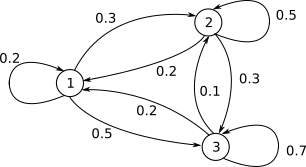
\includegraphics[scale=1.0]{images/markov_1_1.png}
\end{figure}

The corresponding transition probability matrix is therefore

\bee
P = \begin{pmatrix} 0.2 & 0.3 & 0.5 \\
  0.2 & 0.5 & 0.3 \\
  0.2 & 0.1 & 0.7
  \end{pmatrix}
\eee

\subsection{Chapman-Kolmogorov Equations}

A sequence of states visited by the chain is called a sample path. The probability for a sample path is given as follows

\bee
P(X_{n+m}=a, X_{n+m-1}=b, \ldots, X_{n+1}=j | X_n = i) = p_{ij}p_{jk}\cdots p_{cb}p_{ba}
\eee

We next restrict to the probability of sample paths with defined length, ending in state $k$ and starting in state $i$. As an example consider length $2$. Then the probability for a specific sample path (which goes via state $j$) is

\bee
P(X_{2}=k, X_{1}=j | X_{0}=i) = p_{ij}p_{jk}
\eee

If we want the probability $p_{ik}^{(2)}$ of all sample paths with length $2$ which starting in state $i$ and end in state $k$, we sum the probabilities of all states in between; i.e.

\be\label{20190207:eq1}
p_{ik}^{(2)} = \sum_j P(X_{2}=k, X_{1}=j | X_{0}=i) = \sum_j p_{ij}p_{jk}
\ee

We can extend this calculation to longer sample paths

\bee
p_{il}^{(3)} = \sum_j \sum_k p_{ij}p_{jk}p_{kl} = \sum_j p_{ij} p_{jl}^{(2)}
\eee

and also rewrite it as follows

\bee
p_{il}^{(3)} = p_{ij}p_{jk}p_{kl} = \sum_j p_{ij} p_{jl}^{(2)} = \sum_k p^{(2)}_{ik} p_{kl}
\eee

We can collect the $p_{ik}^{(2)}$ in a matrix $P^{(2)}$ which is connected to $P$ via

\bee
P^{(2)} = P^2
\eee

Here the summation across the nodes in between (\eqref{20190207:eq1}) is done implicitely by the matrix multiplication. Of course, this generalizes to longer paths as

\bee
P^{(N)} = P^N
\eee

Let $\pi^{(n)}$ denote the row vector containing the Markov state probabilities $P(X_n)$, we have

\bee
\pi^{(1)} = \pi^{(0)} P
\eee

Note that we need to multiply the vector from the left with the matrix. By an induction argument we can extend this to

\bee
\pi^{(N)} = \pi^{(0)} P^N
\eee

We can take the limit $\lim_{N \rightarrow \infty} P^N$: If it exists then all rows are the same. This shows that $\pi^{(N)}$ becomes independent of the initial state. In our example the limit exists and equals

\bee
\lim_{N \rightarrow \infty} P^N = \begin{pmatrix}
0.2  & 0.233351  & 0.566649 \\
0.2  & 0.233351  & 0.566649 \\
0.2  & 0.233351  & 0.566649
\end{pmatrix}
\eee

\subsection{Sojurn Time}

In the example Markov chain above, the diagonal elements of $P$ are all non-zero and smaller than $1$. Therefore, the chain may stay in the current state or leave it. The number of consecutive time periods that a Markov chain stays in the same state is called sojurn time or holding time.

Let $R_i$ denote the sojurn time for state $i$ and it can be calculated as follows: If the chain is in state $i$, it will stays in this state with probability $p_{ii}$ and leave to another state with probability

\bee
\sum_{j \neq i} p_{ij} = 1 - p_{ii}
\eee

This can be interpreted as Bernoulli trial and the probability for $R_i$ is a geometric distribution with

\bee
P\{R_i = k\} = (1-p_{ii})p^{k-1}_{ii}
\eee

The expected value of $R_i$ is therefore

\bee
E\{R_i\} = \frac{1}{1-p_{ii}}
\eee


\subsection{State Classification}

\begin{description}
\item Transient state: The Markov chain can enter and leave these states for a number of states but it will not stay in transient states forever.

\item Ephemeral state: These are transient states which do not exist beyond the initial time step.

\item Reccurent state: Once entered, the Markov chain will never leave recurrent states. Note that these can also be periodic; i.e. the Markov chain will move between two or more recurrent states.

\end{description}

In the example below, states $1,$ are ephermal transient states, $3,4,5$ are transient states, and $6,7,8$ are recurrent states. Note that states $6,7$ are periodic (once in one of the states, the Markov chain periodically moves between these two states). On the contrary, when the chain has reached state $8$, it will stay in this state.


\begin{figure}[H]
  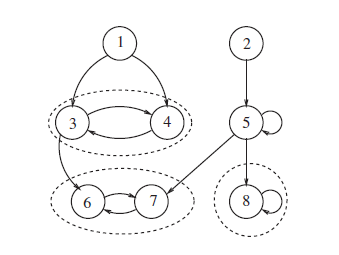
\includegraphics[scale=1.0]{images/markov_1_2.png}
\end{figure}


\subsection{Irreducibility}

After the classification of individual states we classify sets of states. Let $S$ denote all states of a Markov chain, and $S-1, S_2$ two subsets partitioning $S$. $S_1$ is said to be closed, when no one-step transition from $S_1$ to $S_2$ is possible. In our runing example, the set of states $6,7$ are closed, as is the (one-element) set $8$.

A state $j$ is reachable from state $i$, if there exists a path from state $j$ to $i$. This is written as $i \rightarrow j$. State $3$ is reachable from state $1$, but not the other way round. States $3$ and $4$ are reachable from each other. A Markov chain is irreducible, if every state os reachable from every other state; i.e. there exists an integer $n$, for which $p^{(n)}_{ij} > 0$ for all $i,j$.

If $i \rightarrow j$ and $j \rightarrow i$, then the states are said to be communicating states and we write $i \leftrightarrow j$. This property is symmetric, transitive, and reflexive and is therefore an equvalence relationship. A state that communicates with itself is a return state, one that does not communicate with itself is a nonreturn state. Once a Markov chain leaves a nonreturn state, it will never return. The set of all states communicating with state $i$ forms a class which is denoted by $C(i)$.



\subsection{Potential, Fundamental, and Reachability Matrices}

Let $r_{ij}$ be the expected number of times that state $j$ is visited, given that the chain starts in chain $i$. We collect all these values into a matrix $R$ called the potential matrix which can be calculated as

\bee
R = \sum_{n=0}^\infty P^n
\eee

To gain further insight, we rearrange the states so that the transient states come before the recurrent ones. This allows partitioning the matrix $P$ according to

\be\label{20190207:eq2}
P = \begin{pmatrix} T & U \\ 0 & V\end{pmatrix}
\ee

The matrix $T$ represents state transitions between transient states, the matrix $U$ represents state transitions from transient states to recurrent ones, and the matrix $V$ represents state transitions between recurrent states.

For the Markov chain in the Figure above, the matrix $P$ could have the following partitioned form

\bee
P = \left(\begin{array}{ccccc|ccc}
      0 & 0   & 0.5 & 0.5 & 0   & 0    &   0   & 0    \\
      0 & 0   & 0   & 0   & 1    &   0   & 0   &  0   \\
      0 & 0   & 0   & 0.3 & 0    &   0.7 & 0   &  0   \\
      0 & 0   & 1   & 0   & 0    &   0   & 0   & 0    \\
      0 & 0   & 0   & 0   & 0.6  &   0   & 0.2 & 0.2  \\ \hline
      0 & 0   & 0   & 0   & 0    &   0   & 1   &  0   \\
      0 & 0   & 0   & 0   & 0    &   1   & 0   &  0   \\
      0 & 0   & 0   & 0   & 0    &   0   & 0   &  1                    
\end{array}\right)
\eee

Note that the $T$ and $V$ matrices are quadratic (as they describe transitions between the same classes of states), wheras $U$ is generally not quadratic as the number of transient states is unequal the number of recurrent states. Also note that the row sums of $T$ and $U$ are not $1$, respectively (as the Markov chain moves from transient states o recurrent ones). The row sums of $V$ are $1$ as the chain does not leave recurrent states anymore.

We consider a state $i$ and the elements on row $i$: Depending on the classification of states, several possibilities occur.

\paragraph{Recurrent state $i$.} When a state $i$ is recurrent, the Markoc chain returns to it an infinite number of times. Therefore $r_{ii} = \infty$. Furthermore, for $j$ of the states communicating with $i$ (the class $C(i)$) are also $r_{ij} = \infty$. All other row elements are zero. All in all, we have

\bee
r_{ij} = \begin{cases} \infty, \quad & j \in C(i) \\ 0 \quad & \text{otherwise} \end{cases}
\eee

\paragraph{Transient state $i$, recurrent state $j$.}

If a transient state $i$ can reach any state $k$ in the recurrent class $C(j)$, then $r_{ik} = \infty$. Reaching ``any state'' means, that there is an $n$, for which $p^{(n)}_{ij} > 0$.

If the transient state cannot reach any state in $C(j)$, then

\bee
r_{ik} = 0, \quad k \in C(j)
\eee

\paragraph{Transient states $i$ and $j$.} In this case, we calculate $P^n$ by means of the partitioned $P$ \eqref{20190207:eq2} first,

\bee
P^n  = \begin{pmatrix} T^n & \tilde{U}(n) \\0 & V^n \end{pmatrix}
\eee

and insert this into the definition of $R$,

\bee
R = \sum_{n=0}^\infty P^n = \begin{pmatrix}\sum_n T^n & \sum_n \tilde{U}(n) \\ 0 & \sum_n V^n  \end{pmatrix}
\eee

where $\tilde{U}(n)$ is some matrix (depending on $n$). We define the fundamental matrix $S = \sum_n T^n$. The $r_{ij}$ in this matrix $S$ are the only elements which are different from zero or infinity. The $ij$-th element of $S$ gives the expected number of times the chain is in transient state $j$ when it started in transient state $i$.

The fundamental matrix $S$ can be obtained by

\bee
S = I + T + T^2 + T^3 + \cdots = (I - T)^{-1}
\eee



%%% Local Variables:
%%% mode: latex
%%% TeX-master: "journal"
%%% End:
